\bookchapter{الفصل 60: تجهيز بيئة التطوير — Xcode وأول مشروع}

\chapterintro{من أراد أن يُتقن عمله أتقن أدواته أولاً. في هذا الفصل سنجهز «المطبخ»: نثبّت Xcode ونشغّل المحاكي وننشئ أول مشروع iOS في حياتك، ثم نفكك بنية المشروع نفهمها فهماً تاماً. وبعد تجهيز البيئة سترى لأول مرة كودك يتحول إلى زر يمكن النقر عليه — لحظة يتذكرها كثير من الناس طول العمر.}

\booksection{أولاً: تجهيز جهاز Mac}

لنبدأ بالعقبة: تطوير iOS لا يكون إلا على macOS. إن لم تكن تملك Mac فخياراتك ثلاثة: شراء جهاز (يكفي Mac mini أو MacBook Air حتى مستعملاً)، أو استئجار Mac سحابي لفترة قصيرة، أو قراءة القسم الثامن أولاً «التطبيق العملي لتطوير Android» (يمكن العمل عليه من Windows).

\begin{center}
\begin{tabularx}{\linewidth}{|X|X|X|}
\hline
\textbf{بند الإعداد} & \textbf{الحد الأدنى} & \textbf{المستوى المريح (موصى به)} \tabularnewline
\hline
الشريحة & Apple Silicon (من M1 فصاعداً) & M2 وأحدث \tabularnewline
الذاكرة & 8GB & 16GB \tabularnewline
القرص & احجز 40 غيغابايت فأكثر (فـ Xcode نفسه ضخم) & 256 غيغابايت على الأقل \tabularnewline
النظام & أحدث macOS & فعّل التحديث التلقائي \tabularnewline
\hline
\end{tabularx}
\end{center}

\begin{center}\small\color{gray}مرجع مواصفات جهاز تطوير Mac (أغسطس 2026)\end{center}

\begin{tcbinfo}{نصيحة: يمكن تعلم اللغة أولاً دون Mac}
تطبيق Swift Playgrounds المجاني على iPad يتيح تعلم أساسيات لغة Swift (دون حاجة إلى Mac)؛ بل يمكن تثبيته حتى على iPhone. أتقن أولاً المعرفة اللغوية للفصل 61 داخل Playgrounds، وعندما تحصل على Mac ستقلع مباشرة. من شحذ فأسه لم يضيّع وقت الحطب — وهذا هو المقصود بالضبط.

\end{tcbinfo}

\booksection{ثانياً: تثبيت Xcode}

Xcode هي بيئة التطوير المتكاملة الرسمية من Apple وهي مجانية. ثلاث خطوات للتثبيت:

\begin{enumerate}
  \item افتح App Store على Mac وابحث عن "Xcode" وانقر التثبيت — انتبه فهو بحجم عدة غيغابايتات، فاختر وقتاً تكون فيه الشبكة سريعة؛
  \item عند أول تشغيل بعد التثبيت وافق على الاتفاقية واترك المكونات تكتمل (يتم تلقائياً)؛
  \item من القائمة Xcode Settings Locations تأكد من اختيار Command Line Tools — فأدوات سطر الأوامر شرط مسبق للعديد من السكربتات والأدوات الخارجية.
\end{enumerate}

\begin{tcbwarn}{تنبيه: «لعبة التوافق» بين الإصدار والنظام}
Xcode الجديد يطالب غالباً بأحدث macOS، بينما Mac القديم يعلق في الإصدارات القديمة. وعند النشر على App Store تطلب Apple بناء التطبيق بـ Xcode أحدث (مع مهلة سماح عادة). فلا تماطل طويلاً في تحديث النظام — مطورو iOS من أكثر الناس تتبعاً للإصدارات الجديدة.

\end{tcbwarn}

\booksection{ثالثاً: إنشاء أول مشروع لك}

افتح Xcode Create New Project اختر iOS قالب App ثم املأ:

\begin{center}
\begin{tabularx}{\linewidth}{|X|X|X|}
\hline
\textbf{بند الإعداد} & \textbf{ماذا تكتب} & \textbf{التوضيح} \tabularnewline
\hline
Product Name & MyFirstApp & اسم التطبيق \tabularnewline
Team & معرّف Apple ID الخاص بك (مجاني) & يستخدم للتوقيع، والحساب الفردي يكفي \tabularnewline
Organization Identifier & com.example & يتحد مع Product Name ليكوّن معرّف الحزمة \tabularnewline
Interface & SwiftUI & إطار خط هذا الكتاب الرئيسي \tabularnewline
Language & Swift & لا يحتاج إلى شرح \tabularnewline
\hline
\end{tabularx}
\end{center}

\begin{center}\small\color{gray}خمسة بنود تملؤها عند إنشاء المشروع\end{center}

بعد النقر على Create سيولّد Xcode مشروعاً يعمل مباشرة. اختر محاكياً من الزاوية العلوية اليسرى (مثل iPhone 17) وانقر > للتشغيل — بعد ثوانٍ تظهر في شاشة المحاكي نافذة مكتوب فيها “Hello, world!”. لقد وُلد أول تطبيق iOS لك.

\booksection{رابعاً: تشريح بنية المشروع — ما وظيفة كل ملف}

على اليسار متصفح المشروع، ويكفي المبتدئ معرفة هذه فقط:

\begin{center}
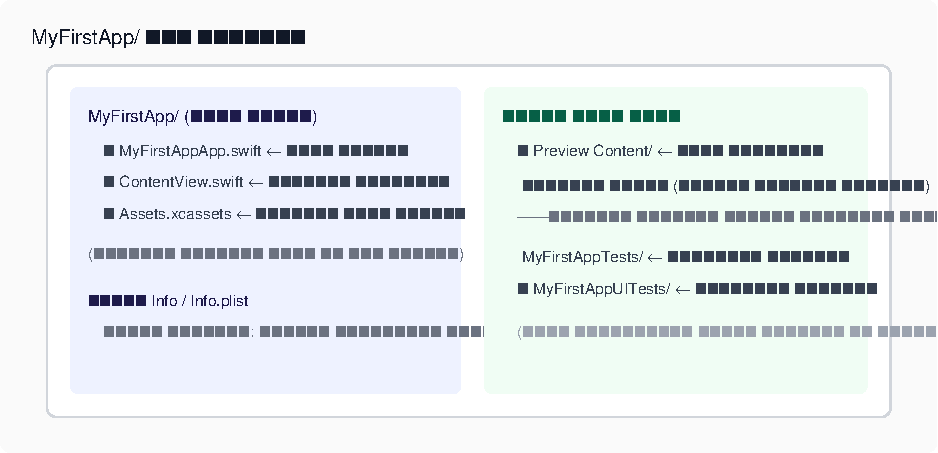
\includegraphics[width=0.92\linewidth]{figures/fig-di-liu-shi-zhang-1}
\\[2pt]\small الشكل 2: بنية مشروع Xcode التي يجب على المبتدئ فهمها
\end{center}

\begin{itemize}
  \item MyFirstAppApp.swift: نقطة دخول البرنامج، وفي SwiftUI لا يتجاوز بضعة أسطر — «ابدأ ثم اعرض الواجهة الرئيسية»؛
  \item ContentView.swift: عرض الواجهة الرئيسية، وكل ما تراه الآن موجود هنا؛
  \item Assets.xcassets: مخزن الموارد — الأيقونات والصور والألوان توضع هنا؛
  \item إعدادات Target: انقر أيقونة المشروع الزرقاء على اليسار للدخول، فداخلها رقم الإصدار وأدنى إصدار iOS والتوقيع. ومن هنا أيضاً تُضبط الاسم الظاهر للتطبيق والأيقونة.
\end{itemize}

\booksection{خامساً: التصحيح على الجهاز الحقيقي — تثبيت التطبيق في iPhone الخاص بك}

\booksection{خامساً: حيل إتقان Xcode — خمس «إضافات اختصارات» للمبتدئ}

أتقن هذه جيداً وستبدو «محترفاً جداً»:

\begin{center}
\begin{tabularx}{\linewidth}{|X|X|X|}
\hline
\textbf{الإجراء} & \textbf{الاختصار} & \textbf{الوظيفة} \tabularnewline
\hline
التشغيل & CmdR & تصريف التطبيق وتشغيله \tabularnewline
فتح/تبديل معاينة اللوحة & OptionCmd & مفتاح «ما تراه هو ما تحصل عليه» \tabularnewline
تنسيق المسافات البادئة & CtrlI & ترتيب مسافات الكود المحدد تلقائياً \tabularnewline
فتح الملفات بسرعة & CmdO & اكتب اسم الملف فيُفتح فوراً (الأكثر استخداماً!) \tabularnewline
تعليق/إلغاء تعليق & Cmd/ & تعطيل وتمكين الأسطر بسرعة أثناء التصحيح \tabularnewline
\hline
\end{tabularx}
\end{center}

\begin{center}\small\color{gray}اختصارات Xcode الأكثر استخداماً (خمسة للمبتدئ)\end{center}

وميزتان خفيتان إضافيتان: تشغيل أكثر من محاكي (لتشغيل iPhone وiPad معاً ومقارنة التخطيط) ومكتبة مقتطفات الكود (اسحب الأسطر الشائعة إلى لوحة Snippets على اليمين لتدرجها لاحقاً بنقرة واحدة) — استخدم أدوات الإتقان من الآن وستتحسن براعتك تلقائياً.

\booksection{سادساً: التصحيح على الجهاز الحقيقي — تثبيت التطبيق في iPhone الخاص بك}

المحاكي جيد لكن الجهاز الحقيقي هو المحطة النهائية. ويمكن التصحيح على جهاز حقيقي بمعرّف Apple ID مجاني:

\begin{enumerate}
  \item وصّل iPhone بكابل البيانات (أو صحّح لاسلكياً عبر شبكة Wi-Fi نفسها)؛
  \item اختر هاتفك من قائمة الأجهزة أعلى Xcode، وفي المرة الأولى سيُطالبك بتسجيل الدخول إلى Apple ID ويضبط التوقيع تلقائياً؛
  \item في iPhone: [الإعدادات] [عام] [VPN وإدارة الأجهزة] ثق بشهادة المطوّر الخاصة بك؛
  \item انقر > فيُثبَّت التطبيق على الجهاز الحقيقي.
\end{enumerate}

\begin{tcbwarn}{تنبيه: «قيد الأيام السبعة» للحساب المجاني}
التطبيق الموقّع بمعرّف Apple ID مجاني يبطل بعد 7 أيام (يُجدد بمجرد إعادة التشغيل مرة واحدة). هذه آلية Apple لمنع إساءة الاستخدام وتكفي تماماً في مرحلة التعلم؛ أما حساب المطور المدفوع (99 دولاراً في السنة) فلا يخضع لهذا القيد، والتفصيل في الفصل 67.

\end{tcbwarn}

\booksection{سابعاً: أول تجربة + إسعاف الأخطاء الشائعة}

\booksection{تاسعاً: أول تجربة + إسعاف الأخطاء الشائعة}

افتح ContentView.swift واستبدل الكلمة في Text(“Hello, world!”) باسمك واضغط CmdR لإعادة التشغيل — بعد ثوانٍ سيظهر اسمك على المحاكي. مبروك، لقد أتممت أول دورة كاملة «تعديل الكود التصريف التثبيت التشغيل».

\begin{center}
\begin{tabularx}{\linewidth}{|X|X|X|}
\hline
\textbf{ظاهرة الخطأ} & \textbf{السبب الشائع} & \textbf{العلاج} \tabularnewline
\hline
خطأ Signing & عدم اختيار Team أو انتهاء صلاحية الشهادة & فعّل حسابك في Target Signing؛ وأعد التشغيل مرة واحدة للحساب المجاني \tabularnewline
شاشة المحاكي سوداء أو لا يفتح & صورة النظام تالفة & من القائمة Device Erase All Content؛ أو احذف المحاكي وأضفه من جديد \tabularnewline
تحميل Xcode بطيء أو يفشل التثبيت & تذبذب الشبكة في App Store & جرّب وقتاً آخر؛ أو نزّل حزمة .xip دون اتصال من موقع مطوري Apple \tabularnewline
\hline
\end{tabularx}
\end{center}

\begin{center}\small\color{gray}جدول إسعاف أخطاء البيئة للمبتدئين\end{center}

\begin{tcbpractice}{لنطبّق: أتمم قائمة «طقوس التطوير» الخاصة بك}
(1) ثبّت Xcode وشغّل المحاكي بنجاح؛ (2) شغّل تطبيقك على جهاز حقيقي مرة والتقط صورة تذكارية؛ (3) استبدل كلمة Hello باسمك؛ (4) من إعدادات Target غيّر الاسم الظاهر للتطبيق إلى «تطبيقي الأول». بإتمام هذه الخطوات الأربع تصبح صاحب عمل منجز.

\end{tcbpractice}

\begin{tcbsummary}{خلاصة الفصل}
\begin{itemize}
  \item العقبة الصلبة: Mac + Xcode؛ وإن لم يتوفر Mac فتعلم اللغة أولاً عبر Swift Playgrounds على iPad
  \item ثبّت Xcode من App Store؛ الإصدار الجديد يطالب بنظام جديد، فلا تماطل في التحديث
  \item عناصر المشروع الجديد الخمسة: الاسم وTeam ومعرّف المؤسسة وSwiftUI وSwift
  \item قاعدة المشروع: الكود كله في مجلد MyFirstApp/؛ وإعدادات Target تتكفل بالإصدار والتوقيع
  \item التصحيح على جهاز حقيقي بمعرّف Apple ID مجاني خاضع لقيد توقيع 7 أيام؛ والحساب المدفوع بلا هذا القيد
  \item روتين التطوير = عدّل الكود CmdR شاهد النتيجة، في دورة متجددة
\end{itemize}

\end{tcbsummary}
